%-----------------------------------------------------------------------------------------------%
%
% Maret 2019
% Template Latex untuk Tugas Akhir Program Studi Sistem informasi ini
% dikembangkan oleh Inggih Permana (inggihjava@gmail.com)
%
% Template ini dikembangkan dari template yang dibuat oleh Andreas Febrian (Fasilkom UI 2003).
%
% Orang yang cerdas adalah orang yang paling banyak mengingat kematian.
%
%-----------------------------------------------------------------------------------------------%


%-----------------------------------------------------------------------------%
\chapter{\babTiga}
%-----------------------------------------------------------------------------%
Kerangka penelitian ini adalah langkah demi langkah dalam penyusunan Tugas Akhir mulai dari Tahap Perencanaan penelitian hingga Tahap Hasil dan Dokumentasi. Berikut ini adalah gambar Metodologi Penelitian dapat dilihat pada Gambar 3.1.
\begin{figure}
	\centering
	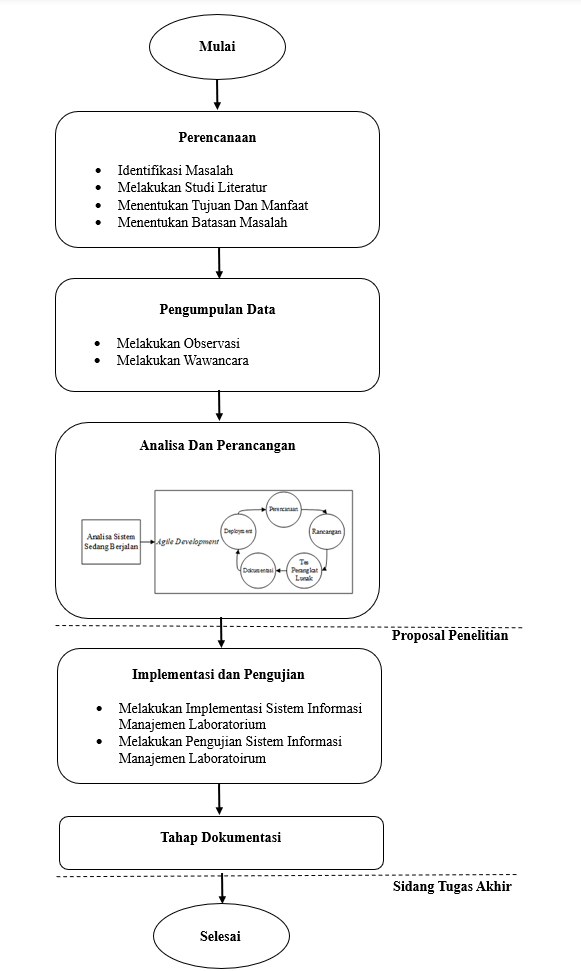
\includegraphics[width=0.82\linewidth]{konten//gambar/metodologi-penelitian.png}
	\caption{Metodologi Penelitian}
	\label{fig:enter-label}
\end{figure}
%-----------------------------------------------------------------------------%
\section{Tahap Perencanaan}
Langkah pertama dalam penelitian ini adalah mengidentifikasi masalah, studi literatur, menentukan tujuan dan manfaat, menentukan batasan masalah, menentukan data-data serta informasi yang dibutuhkan saat penelitian.

\subsection{Identifikasi Masalah}
Pada tahap ini, tujuan dari penelitian ini adalah untuk menemukan masalah dalam SITARIS SI untuk digunakan sebagai rumusan masalah. Dari masalah yang telah ditemukan dan disebutkan sebelumnya, rumusan masalah yang dihasilkan dari penelitian ini adalah “Bagaimana mengevaluasi kualitas SITARIS SI menggunakan metode ISO 9126 untuk dapat menentukan tingkat kualitas sistem dan kemudahan akses bagi pengguna serta memberikan rekomendasi untuk pengembangan sistem selanjutnya”.

\subsection{Studi Literatur}
Pada tahap ini, hal pertama yang dilakukan adalah melakukan penelitian literatur untuk mendapatkan informasi yang diperlukan untuk menulis tentang topik yang diangkat. Selain itu, kegiatan penelitian ini juga membantu mengetahui teori teori, serta metode dan teknik yang berkaitan dengan topik atau masalah yang akan digunakan untuk mencapai tujuan yang diinginkan. Teori yang digunakan di sini berasal dari artikel jurnal.

\subsection{Menentukan Tujuan dan Manfaat}
Pada tahap ini, akan dibahas tentang rumusan kalimat yang menunjukkan adanya hasil, tujuan penelitian, dan apa yang diperoleh setelah penelitian selesai.

\subsection{Menentukan Batasan Masalah}
Pada tahap ini, yang dilakukan adalah membatasi subjek penelitian. Untuk mengumpulkan masalah, penelitian ini menggunakan wawancardan dan kuisioner. Penelitian ini menggunakan metode Model ISO 9126 untuk menganalisis kualitas. Penelitian ini menggunakan teknik Probability Sampling, yaitu Proportionate Stratified Random Sampling, dan rumus slovin digunakan untuk menghitung jumlah sampel.

\section{Tahap Pengumpulan Data}
Langkah kedua dalam penelitian ini adalah menghimpun data baik data primer maupun data sekunder melalui kegiatan wawancara dan penyebaran kuesioner.

\subsection{Melakukan Wawancara}
Wawancara merupakan teknik pengumpulan data yang dilakukan melalui tatap muka dan tanya jawab langsung antara peneliti dan narasumber. Wawancara dilakukan untuk mendapatkan informasi secara tepat dan akurat dari narasumber yang terpercaya. Narasumber yang terkait pada penelitian ini yaitu bapak Tengku Khairil Ahsyar S.Kom., M.Kom., selaku Kepala Laboratorium Sistem Informasi.

\subsection{Menentukan Populasi dan Sampel}
Penentuan populasi dan sampel merupakan langkah krusial dalam penelitian ini, karena akan mempengaruhi validitas dan reliabilitas hasil evaluasi SITARIS SI. Proses ini dilakukan dengan cermat untuk memastikan bahwa sampel yang dipilih dapat merepresentasikan keseluruhan populasi pengguna sistem dengan akurat. Populasi dalam penelitian ini mencakup seluruh pengguna SITARIS SI di UIN Suska Riau. Berdasarkan informasi yang diberikan sebelumnya, populasi ini terdiri dari dua kelompok utama, yaitu:

\begin{enumerate}
	\item Staff laboratorium: Kelompok ini mencakup semua personel yang bekerja di laboratorium dan menggunakan SITARIS SI dalam tugas sehari-hari mereka seperti Kepala Laboratorium dan Asisten Laboratorium.
	\item Mahasiswa: Kelompok ini terdiri dari mahasiswa UIN Suska Riau yang menggunakan SITARIS SI untuk keperluan akademik mereka seperti peminjaman ruangan dan barang.
\end{enumerate}

Jumlah total populasi akan ditentukan berdasarkan data terbaru dari administrasi universitas mengenai jumlah staff laboratorium dan mahasiswa yang terdaftar sebagai pengguna SITARIS SI. Untuk penelitian ini, digunakan teknik \textit{Probability Sampling}, khususnya metode \textit{Proportionate Stratified Random Sampling}. Metode ini dipilih karena beberapa alasan:

\begin{enumerate}
	\item Populasi terdiri dari dua kelompok yang berbeda (staff dan mahasiswa), yang masing-masing mungkin memiliki perspektif dan pengalaman yang berbeda dengan SITARIS SI.
	\item Metode ini memungkinkan representasi yang proporsional dari kedua kelompok dalam sampel final, sehingga menjamin bahwa pandangan dari kedua kelompok akan tercermin dalam hasil penelitian.
	\item Penggunaan \textit{random sampling} dalam setiap strata (kelompok) membantu mengurangi bias dan meningkatkan validitas hasil penelitian.
\end{enumerate}

Untuk menentukan ukuran sampel yang tepat, penelitian ini menggunakan rumus Slovin. Rumus ini dipilih karena kemampuannya untuk menentukan ukuran sampel yang representatif dari populasi yang diketahui dengan tingkat kesalahan yang dapat ditoleransi. Rumus Slovin adalah sebagai berikut:

\[ n = \frac{N}{1 + N \cdot e^2} \] \\

Di mana:

n = ukuran sampel

N = ukuran populasi

e = margin error \\

Untuk penelitian ini, margin error yang digunakan adalah 5\% (0,05), yang merupakan standar umum dalam penelitian sosial. Setelah ukuran sampel total ditentukan, jumlah sampel untuk setiap strata (staff laboratorium dan mahasiswa) akan dihitung secara proporsional berdasarkan persentase mereka dalam populasi total.

Setelah jumlah sampel untuk setiap strata ditentukan, proses pengambilan sampel acak akan dilakukan dalam setiap strata. Ini bisa dilakukan dengan menggunakan tabel angka acak atau software penghasil angka acak untuk memilih responden dari daftar lengkap populasi dalam setiap strata.
Dengan menggunakan metode ini, penelitian ini bertujuan untuk mendapatkan sampel yang representatif dan seimbang, yang akan memberikan wawasan yang akurat tentang persepsi dan pengalaman pengguna SITARIS SI di UIN Suska Riau.

\subsection{Membuat dan Menyebarkan Kuisioner}
Peneliti melakukan penyebaran kuisioner berdasarkan faktor atau karakteristik sesuai terkait evaluasi SITARIS SI ini. Setiap karakteristik memiliki sub karakteristik, masing– masing dari sub karakteristik yang nantinya akan disebarkan kepada responden. Responden yang terkait pada SITARIS SI adalah staff laboratorium dan mahasiswa UIN Suska Riau.

\section{Tahap Analisis dan Hasil}
Langkah ketiga dalam penelitian ini adalah menganalisis SITARIS SI, menganalisis Pengolahan Kuisioner, menganalisis Pengukuran Model ISO 9126.

\subsection{Menganalisis SITARIS SI}
Analisis SITARIS SI merupakan tahap krusial dalam evaluasi sistem. Proses ini melibatkan pemeriksaan menyeluruh terhadap berbagai aspek sistem untuk memastikan kualitas dan efektivitasnya.

Langkah pertama dalam evaluasi ini adalah evaluasi fungsionalitas sistem. Peneliti akan memeriksa setiap fitur SITARIS SI untuk memastikan bahwa semua berfungsi sesuai dengan spesifikasi yang telah ditentukan. Ini mencakup pengujian setiap modul, menu, dan fungsi dalam sistem untuk memverifikasi bahwa mereka beroperasi dengan benar dan memberikan output yang diharapkan.

Selanjutnya, antarmuka pengguna akan dievaluasi dari segi kegunaan dan kemudahan penggunaan. Aspek ini sangat penting karena berdampak langsung pada pengalaman pengguna dan efisiensi operasional. Peneliti akan menilai desain antarmuka, navigasi, dan alur kerja untuk memastikan bahwa pengguna dapat dengan mudah memahami dan menggunakan sistem tanpa kebingungan atau frustrasi.

Performa sistem juga menjadi fokus utama dalam evaluasi ini. Peneliti akan mengukur kecepatan respons sistem dalam berbagai skenario penggunaan, serta mengevaluasi efisiensinya dalam mengelola data. Ini melibatkan pengujian kinerja sistem under load, menganalisis waktu respons untuk berbagai operasi, dan menilai kemampuan sistem dalam menangani volume data yang besar.

Aspek keamanan SITARIS SI juga akan dievaluasi secara mendalam. Peneliti akan menilai mekanisme keamanan yang diterapkan untuk melindungi data sensitif, termasuk manajemen akses pengguna, dan perlindungan terhadap potensi ancaman keamanan. Ini penting untuk memastikan integritas dan kerahasiaan data yang dikelola oleh sistem.

Terakhir, Peneliti akan mengevaluasi bagaimana SITARIS SI terintegrasi dengan sistem lain yang relevan. Ini mencakup pemeriksaan antarmuka dan protokol komunikasi yang digunakan untuk pertukaran data dengan sistem eksternal, serta menilai keefektifan dan efisiensi proses integrasi ini.

\subsection{Menganalisis Pengolahan Kuisioner}
Analisis pengolahan kuisioner adalah langkah penting dalam mengumpulkan dan menginterpretasikan umpan balik pengguna tentang SITARIS SI. Proses ini melibatkan beberapa tahap yang sistematis untuk memastikan bahwa data yang dikumpulkan dapat memberikan wawasan yang bermakna.

Tahap pertama dalam proses ini adalah tabulasi data. Semua respons dari kuisioner yang telah dikumpulkan akan dikompilasi ke dalam format yang terstruktur dan dapat dianalisis. Ini melibatkan penggunaan perangkat lunak Microsoft Excel atau alat analisis statistik khusus seperti SPSS.

Peneliti akan melakukan analisis statistik deskriptif setelah data ditabulasi. Ini melibatkan perhitungan frekuensi, mean, median, dan modus untuk setiap item dalam kuisioner. Analisis ini akan memberikan gambaran umum tentang distribusi respons dan tren dalam data.

Setelah itu, analisis reliabilitas kuisioner akan dilakukan. Ini akan melibatkan penggunaan alat seperti Cronbach's Alpha untuk mengevaluasi seberapa konsisten bagian-bagian dalam kuisioner. Ini sangat penting untuk memastikan bahwa kuisioner secara konsisten mengukur apa yang dimaksudkan untuk diukur.

Selain itu, peneliti akan melakukan analisis validitas untuk memastikan bahwa pertanyaan-pertanyaan dalam kuisioner secara akurat mengukur elemen yang dimaksud. Ini dapat mencakup metode seperti analisis faktor atau validasi konten oleh pakar di bidang tersebut.

Terakhir, hasil statistik akan dipahami dengan mempertimbangkan tujuan penelitian. Peneliti akan mencari pola, tren, atau hasil penting dari data yang dikumpulkan. Interpretasi ini akan membantu memahami bagaimana pengguna melihat SITARIS SI. Ini juga akan membantu menentukan area mana yang perlu diperbaiki atau diperluas.

\subsection{Menganalisis Pengukuran Model ISO 9126}
Untuk menilai kualitas perangkat lunak SITARIS SI, analisis menggunakan model ISO 9126, yang menyediakan kerangka kerja terstruktur yang mencakup enam karakteristik kualitas utama perangkat lunak.

Karakteristik pertama yang akan dievaluasi adalah functionality. Peneliti akan menilai sejauh mana SITARIS SI memenuhi fungsi-fungsi yang dinyatakan dan tersirat dalam spesifikasinya. Ini melibatkan pengujian setiap fitur sistem untuk memastikan bahwa mereka beroperasi sebagaimana mestinya dan memenuhi kebutuhan pengguna.

Reliability sistem juga akan diukur, fokus pada kemampuan SITARIS SI untuk mempertahankan tingkat kinerja tertentu dalam kondisi tertentu. Ini mencakup pengujian ketahanan sistem terhadap kegagalan, kemampuan untuk memperbaiki kesalahan, dan konsistensi kinerja selama periode waktu yang panjang.

Usability SITARIS SI akan dievaluasi untuk menilai seberapa mudah sistem dipelajari, dioperasikan, dan digunakan oleh pengguna. Ini melibatkan pengujian pengguna, analisis antarmuka, dan penilaian dokumentasi sistem.

Efficiency sistem akan diukur dengan menilai kinerja SITARIS SI relatif terhadap sumber daya yang digunakan. Ini mencakup evaluasi waktu respons, penggunaan sumber daya, dan skalabilitas sistem.

Maintainability SITARIS SI akan dianalisis untuk menilai kemudahan sistem untuk dimodifikasi, diperbaiki, atau diadaptasi terhadap perubahan lingkungan. Ini melibatkan pemeriksaan struktur kode, modularitas, dan dokumentasi teknis.

Terakhir, portability sistem akan dievaluasi untuk menilai kemampuan SITARIS SI untuk ditransfer ke lingkungan yang berbeda. Ini mencakup pengujian kompatibilitas dengan berbagai platform atau lingkungan operasi.

Untuk setiap karakteristik ini, tim akan mengukur metrik yang relevan, membandingkannya dengan standar atau benchmark yang sesuai, dan mengidentifikasi area-area yang memerlukan perbaikan. Hasil dari analisis ini akan memberikan gambaran komprehensif tentang kualitas SITARIS SI berdasarkan standar internasional yang diakui.

\section{Tahap Kesimpulan dan Dokumentasi}
Langkah keempat dalam penelitian ini adalah membuat persentase kelayakan sistem, membuat rekomendasi dan kesimpulan.

\subsection{Membuat Persentase Kelayakan Sistem}
Persentase kelayakan website ini merupakan tahap proses untuk mengetahui persentase kelayakan dari sebuah website sehingga dapat ditarik kesimpulan apakah website tersebut termasuk kategori layak atau tidak website tersebut sehingga dapat ditarik kesimpulan apakah website tersebut dapat dikembangkan, dilanjutkan, atau diberhentikan. Besarnya persentase dapat dihitung dengan rumus berikut:

\[
\text{Persentase Kelayakan} = \frac{\text{Skor Aktual}(f)}{\text{Skor Ideal}} \times 100\%
\]

Dari rumus diatas diperoleh dengan cara menghitung skor
aktual (f) yang dibagi dengan skor ideal (n) kemudian dikalikan 100\%. Skor actual sendiri merupakan jumlah skor jawaban dari responden, sedangkan skor ideal (n) merupakan skor tertinggi jika responden tersebut memilih jawaban dengan skor tertinggi.

Selanjutnya persentase karakteristik tersebut akan dijumlah total untuk mendapatkan persentase keseluruhan. Rumus dalam menghitung persentase keseluruhan adalah sebagai berikut:

\[
\bar{x} = \frac{\sum x}{n}
\]

Keterangan :
X =Persentase rata-rata \\
x= Persentase total karakteristik
n =JumlahKarakteristik

Adapun tabel kelayakan menurut kelayakan menurut Arikunto (2008). Berikut tabelnya :

\begin{table}[h!]
	\centering
	\begin{tabular}{cc}
	\hline
	\textbf{Kategori}        & \textbf{Persentase} \\ \hline
	Sangat Baik              & 81\% - 100\%        \\
	Baik                     & 61\% - 80\%         \\
	Cukup Baik               & 41\% - 60\%         \\
	Tidak Baik               & 21\% - 40\%         \\
	Sangat Tidak Baik        & \textless 21\%      \\ \hline
	\end{tabular}
	\end{table}
	
	
\subsection{Membuat Rekomendasi dan Kesimpulan}
Rekomendasi merupakan sebuah proses untuk melakukan saran atau usulan secara keseluruhan berdasarkan berdasarkan faktor atau karakteristik dan metrik yang dilakukan pada penelitian ini dengan menggunakan metode ISO 9126. Hasil rekomendasi pada penelitian ini nantinya akan menjadi masukan atau saran kepada pihak Laboratorium Program Studi Sistem Informasi.
